\section{Sparse LU Decomposition}

We need to solve equation $A=LU$ where $L$ is the lower triangular matrix and $U$ is the upper triangular matrix. The equation we will get for each element of $L$ and $U$ is given in the following:-
\begin{subequations}
    \centering
    \begin{align}
        U_{(i,j)} & = A_{(i,j)} - \sum\limits_{k = 1}^{i-1} L_{(i,k)}U_{(k,j)} \label{eqn:LUD:LUequation0}\\
        L_{(i,j)} & = \frac{A_{(i,j)} - \sum\limits_{k = 1}^{j-1} L_{(i,k)}U_{(k,j)}}{U_{(j,j)}} \label{eqn:LUD:LUequation1}
    \end{align}
    \label{eqn:LUD:LUequation}
\end{subequations}


We can use Gauss–Jordan elimination to factorize the matrix, although for sparse nature matrix would not be efficient. Therefore we need to go through Direct methods of sparse LU Decomposition. There are majorly three kinds of Direct Methods solving Left-looking, Right-Looking, and Crout \cite{crout}. We will be using Gilbert-Peierls Algorithm: A Column-Oriented LU Factorization with partial pivoting.
Symbolic analysis is a process to determine the set of non-zero locations ($\chi$)
in solving the lower triangular system $L_j x = b$, where $J_j$ is a unit diagonal 
lower triangular matrix representing only first ($j-1$) columns. Listing all 
the non-zero locations \(\chi\) gives the numerical computation time proportional to
the number floating point operations i.e. \bigo{f},


\begin{algorithm}[H]
    \caption{Gilbert-Peierls Algorithm: Solving Triangular System $L_j x = b$
        \label{algo:GP_tri}}
    \begin{algorithmic}[1]
        \Require{$L_j$ is a lower triangular matrix, $x, b$ are sparse column vectors}
        \Statex
        \State $x := b$
        \For{$\textrm{ each } j \in \chi$}
            \For{$\textrm{ each } i > j \textrm{ for which } l_{ij} \neq 0$}
                \State $x_i := x_i - l_{ij} x_j$
            \EndFor
        \EndFor
    \end{algorithmic}
\end{algorithm}

\begin{figure}[H]
    \centering
    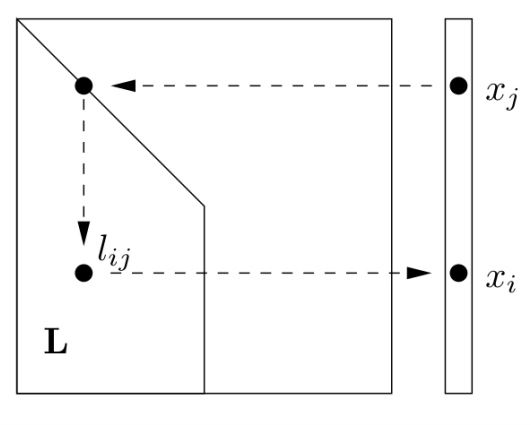
\includegraphics[width = 0.50\textwidth]{./Theory/nnzPattern.JPG}
    \caption{Non-zero pattern in LU decomposition}
    \label{fig:GP:nnzPattern}
\end{figure}

The algorithm suggests that the element of the result vector ($x_{ij}$) can become non-zero only of the corresponding element in the vector $b$ ($b_{i}$) is non-zero or there exits a non-zero element $l_{i,j}$ where $j$ is less than $i$ and $x_{j}$ is non zero. 

\begin{subequations}
    \centering
    \begin{align}
        (b_i \neq 0) &\implies (x_i \neq 0) \\
        (x_j \neq 0) and \exists i(l_{ij} \neq 0) &\implies (x_i \neq 0)
    \end{align}
    \label{eqn:GP:findingX}
\end{subequations}

Symbolic Analysis can visualize these two implications using the figure \ref{fig:GP:nnzPattern}.In the column factorization algorithms like Gilbert-Peierls, we know the locations of all the non-zero elements for the columns with indices lower than $j$ we can determine the non-zero sites ($\chi$) before solving for that column and the entire lower triangular system.


We can consider following example with $10\times10$ in the figure with \ref{fig:SPLsolve0}
\begin{figure}[H]
    \centering
    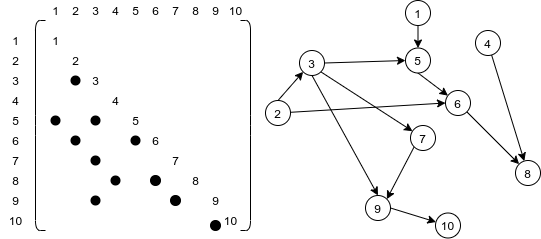
\includegraphics[width = 0.65\textwidth]{./Theory/PpT-SPLsolve0.png}
    \caption{DAG generated for $10\times10$ Sample Matrix}
    \label{fig:SPLsolve0}
\end{figure}

As per the non-zero value obtained from the value of b in $Lx=b$ will be sharing A memory map for the execution of the algorithm \cite{davis2006direct}

